\section{MOS Transistoren}

\subsection{Dotierung}
\begin{center}
    \begin{tabular}{lll}
        \textbf{Dotierung:}          & N-dotiert                & P-dotiert             \\
        \textbf{Unreinheit:}         & Phosphor / Arsen (HG V)  & Aluminium (HG III)    \\
        \textbf{Majoritätsträger:}   & Elektronen               & Löcher                \\
        \textbf{Minoritätsträger:}   & Löcher                   & Elektronen            \\
    \end{tabular}
\end{center}


\subsection{MOS-Kapazität}
\begin{minipage}[t]{0.49\columnwidth}
    Minoritätsträger werden an das Gate gezogen.
    Die entstandene Raumladungszone weist bei ausreichend hoher Gate-Spannung einen Minoritätsträgerüberschuss auf, ist also in der Funktion \textbf{komplementär} zum Substrat dotiert.
\end{minipage}
\hfill
\begin{minipage}[t]{0.49\columnwidth}
    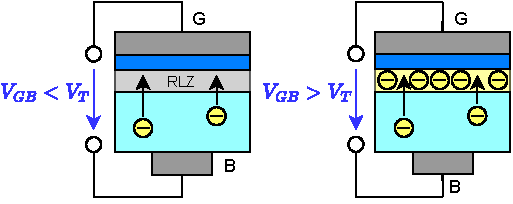
\includegraphics[width=\columnwidth, align=t]{images/02_MOS_kapazitaet.pdf}
\end{minipage}


\subsection{MOS-Transistoren}
Werden links und rechts vom MOS-Kondensator komplementär zum Substrat dotierte Regionen (Drain und Source) erstellt, so kann ohne Gatespannung aufgrund der PN-Übergänge kein Strom vom Drain zur Source (oder umgekehrt) fliessen.
Wird nun eine Spannung am Gate angelegt, so entsteht die Minoritätsträger-Leitende Raumladungszone -- der Kanal.
Dieser verbindet Drain und Source, es kann also ein Strom fliessen.

\vspace{-0.2cm}

\begin{center}
    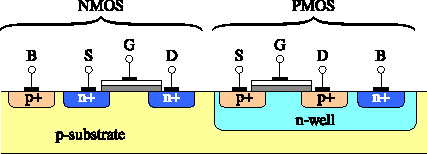
\includegraphics[width=0.5\columnwidth, align=t]{images/02_CMOS.pdf}
\end{center}


\subsubsection{Übersicht und Symbole}

\begin{minipage}[t]{0.48\columnwidth}
    Durch Vordotierung des Kanals kann der Transistor ohne Gate-Spannung leitend gemacht werden (Verarmungstyp, selbstleitend).
    Eine negative Gate-Spannung kann den Kanal dann abschnüren. \\
    \rightarrow\ hier nicht weiter behandelt

    \smallskip

    \textbf{Der Bulk wird nur eingezeichnet, wenn dieser \myul{nicht} mit $\bm{V_{\rm DD}}$ bzw. $\bm{V_{\rm SS}}$ verbunden ist.}
    Deshalb werden meist die vereinfachten Symbole verwendet:

    \vspace{-0.3cm}

    \begin{center}
        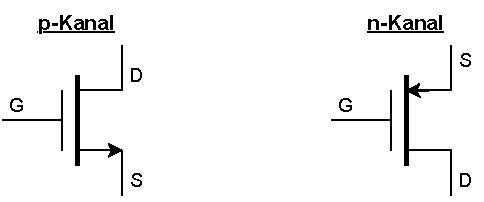
\includegraphics[width=0.8\columnwidth, align=t]{images/02_MOSFET_symbole_vereinfacht.pdf}
    \end{center}
\end{minipage}
\hfill
\begin{minipage}[t]{0.5\columnwidth}
    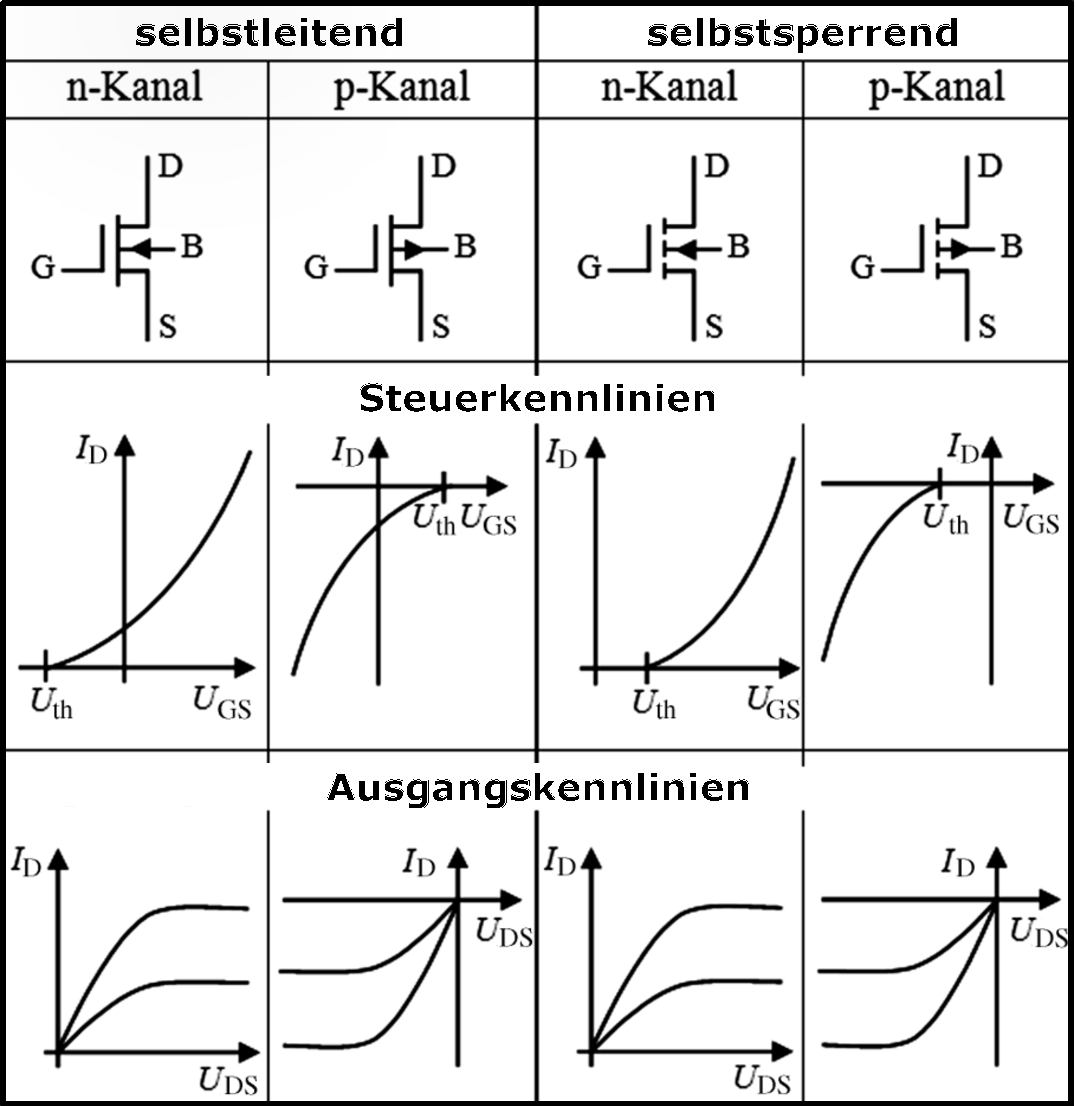
\includegraphics[width=\columnwidth, align=t]{images/02_MOSFET_uebersicht.pdf}
\end{minipage}



\subsubsection{Modelle}
In Cadence sind verschiedene Modelle hinterlegt:

\smallskip
\begin{description}
    \item[Spice Modell 11:] Das Modell 11 beinhaltet ca. 100 Parameter und ist entsprechend genau.
    \item[Spice Modell 1:] Vergleichbar mit dem Handrechenmodell, welches zwar weniger genau, dafür aber viel einfacher ist. Dennoch beinhaltet es bereits 40 Parameter.
\end{description}


\subsection{Ausgangskennlinie -- Arbeitsbereiche}
 
Die Ausgangskennlinie beschreibt den Zusammenhang $I_D = f(V_{\rm DS}) \big|_{V_{\rm GS} = \text{konst}}$

\begin{minipage}[t]{0.5\columnwidth}
    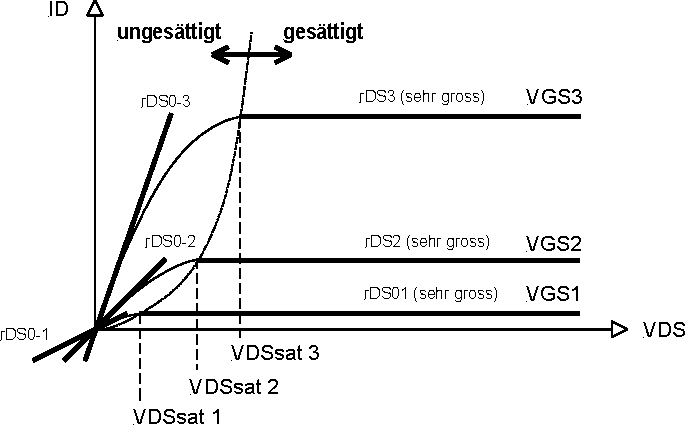
\includegraphics[width=\columnwidth, align=t]{images/02_MOSFET_ausgangskennlinien.pdf}
\end{minipage}
\hfill
\begin{minipage}[t]{0.48\columnwidth}
    Zwei Arbeitsbereiche: 

    \begin{outline}
        \1 ungesättig (gesteuerter Widerstand)
        \1 gesättigt (Stromquelle)
    \end{outline}

    \medskip

    Die Sättigungsgrenze $V_{\rm DS, sat}$ ist abhängig vom \textbf{Kanalzustand}:

    \begin{outline}
        \1 \textbf{weak inversion:} \\
            $V_{\rm DS, sat} = V_{\rm eff} \approx 5 \cdot V_{\rm temp} \approx \qty{130}{\milli \volt}$ 
        \1 \textbf{strong inversion:} \\
            $V_{\rm DS, sat} = V_{\rm eff} = V_{\rm GS} - V_T$ 
    \end{outline}
\end{minipage}



\subsection{Transferkennlinie -- Ausgangsstrombereiche}


\begin{minipage}[t]{0.55\columnwidth}
    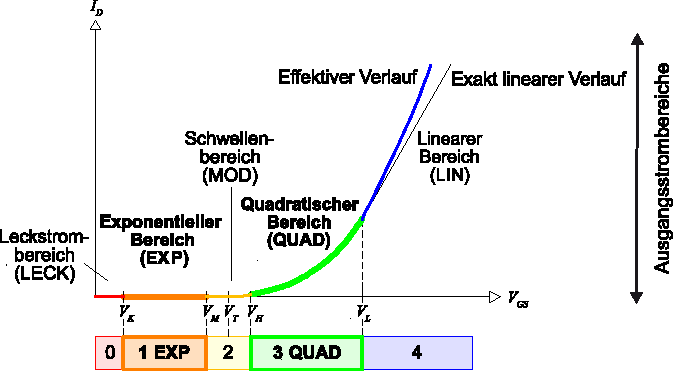
\includegraphics[width=\columnwidth, align=t]{images/02_MOSFET_transferkennlinie.pdf}
\end{minipage}
\hfill
\begin{minipage}[t]{0.42\columnwidth}
    Die Transferkennlinie beschreibt den Zusammenhang $I_D = f(V_{\rm GS})$ 

    \smallskip

    Dabei werden \textbf{5 Ausgangsstombereiche} unterschieden. Diese hängen mit dem \textbf{Kanalzustand} zusammen.

    \smallskip

    Des Weiteren gibt es die Bereiche:

    \begin{outline}
        \1 Sub Threshold: $V_{\rm GS} < V_T$
        \1 Above Threshold: $V_{\rm GS} > V_T$
    \end{outline}
\end{minipage}


\paragraph{Ausgangsstrombereiche}

\scalebox{0.8}{
\begin{tabular}{|l|l|l|}
    \hline
    \textbf{Bereich}                    & \textbf{Mathem. Charakterisierung}            & \textbf{Zugrundeliegender phys. Effekt}                       \\  
    \hline
    \rowcolor[HTML]{F4CCCC} 
    LECK                                & $I_D$ erreicht Minimalwert, der nicht         & Drain- und Source-Substratdiode haben                         \\
    \rowcolor[HTML]{F4CCCC} 
                                        & weiter unterschritten werden kann             & Leckströme ins Subsstrat                                      \\
    \hline
    \rowcolor[HTML]{FFE5BB} 
    EXP                                 & $I_D$ steigt exponentiell mit $V_{\rm GS}$        & Kanal zeigt \textbf{weak inversion}                           \\
    \hline
    \rowcolor[HTML]{FFF2CC} 
    MOD                                 & Keine 'handliche' Formel für $I_D$            & Kanal zeigt \textbf{moderate inversion}                       \\
    \hline
    \rowcolor[HTML]{D9EAD3} 
    QUAD                                & $I_D$ steigt quadratisch mit $V_{\rm GS}$         & Kanal zeigt \textbf{strong inversion}                         \\
    \hline
    \rowcolor[HTML]{CFE2F3} 
    LIN                                 & $I_D$ steigt annähernd linear mit $V_{\rm GS}$    & Geschwindigkeitssättigung der Ladungsträger im Kanal          \\
    \rowcolor[HTML]{CFE2F3} 
                                        & (halb QUAD, halb LIN)                         & im Kanal (nicht weiter beschleunigbar)                        \\
    \hline
\end{tabular}
}

\smallskip

\textbf{Hinweis:} Die Inversion des Kanals beschreibt, wie sehr sich die Polarität geändert ('invertiert') hat. 
Bei einem n-Kanal FET ist der Kanal ursprünglich p-leidend.
Wird der Kanal invertiert, so wird er (schwach, moderat oder start) n-leitend. 


\subsection{Berechnung des Drainstroms}

Die Berechnung des Drainstroms hängt sowohl von Arbeitsbereich (gesättigt / ungesättig), als auch vom Ausgangsstrombereich (bzw. der Kanaliversion) ab!


\subsubsection{Strong Inversion}
\label{Strong Inversion}

\vspace{-0.3cm}

% $$ \boxed{ \text{QUAD-Bereich: } V_H(I_D) < V_{\rm GS} < V_L(I_D) } \qquad \qquad \beta = \mu \cdot C_{\text{OX}} \cdot \frac{W}{L} $$
\[ \boxed{ \text{QUAD-Bereich:} \quad |V_H(I_D)| \leq |V_{\rm GS}| < |V_L(I_D)| \quad \text{bzw.} \quad |I_H'| \leq |I_D'| < |I_L'| } \] 

\resizebox{\columnwidth}{!}
{
    \renewcommand{\arraystretch}{1.5}
    \begin{tabular}{@{}l c | c@{}}
                & \textbf{Ungesättigt:} \quad $\bm{| V_{\rm DS} | < | V_{\rm GS} - V_T |}$                                                              & \textbf{Gesättigt:} \quad $\bm{| V_{\rm DS} | \geq | V_{\rm GS} - V_T |}$                         \\
        NMOS:   & $I_D = \beta \cdot \bigg[ (V_{\rm GS} - V_T) V_{\rm DS} - \frac{V_{\rm DS}^2}{2} \bigg] \cbl{\cdot (1 + \lambda \cdot \Delta V_{\rm DS})}$    & $I_D = \frac{\beta}{2} (V_{\rm GS} - V_T)^2 \cbl{\cdot (1 + \lambda \cdot \Delta V_{\rm DS})}$    \\
        \midrule
        PMOS:   & $I_D = - \beta \cdot \bigg[ (V_{\rm GS} - V_T) V_{\rm DS} - \frac{V_{\rm DS}^2}{2} \bigg] \cbl{\cdot (1 - \lambda \cdot \Delta V_{\rm DS})}$  & $I_{D} = - \frac{\beta}{2} (V_{\rm GS} - V_T)^2 \cbl{\cdot (1 - \lambda \cdot \Delta V_{\rm DS})}$
    \end{tabular}
    \renewcommand{\arraystretch}{1}
}

\medskip

\textbf{Ohne} Berücksichtigung der \textbf{Kanallängenmodulation:} \cbl{blauen Term $=1$} bzw $\lambda = 0$ setzen



\paragraph{Transkonduktanz-Parameter $\bm{\beta}$}

\begin{minipage}[c]{0.78\columnwidth}
    $\beta$ ist abhängig davon, ob der Transistor gesättigt ist. 
    In der Praxis wird diese Unterscheidung jedoch \textbf{nicht} gemacht. 
    Im \textbf{Design} kann $\beta$ durch das Verhältnis von Kanalbreite $W$ und -länge $L$ beeinflusst werden.
\end{minipage}
\hfill
\begin{minipage}[c]{0.2\columnwidth}
    \[ \beta = \underbrace{ \mu C_{\rm ox} }_{\beta_0} \frac{W}{L} \]
\end{minipage}

\paragraph{Kanallängenmodulation $\bm{\lambda$} und Early-Spannung $\bm{V_E}$}

% Die Early-Spannung $V_E = a_E \cdot L$ setzt sich zusammen aus dem technologieabhängigen Early-Faktor $a_E$ und der Kanallänge $L$.
Die Kanallängenmodulation beschreibt die Nichtidealität der spannungsgesteurten Stromquelle (im Sättigungsbetrieb).

$$ \lambda = \frac{1}{V_E + V_{\rm DS,  sat}} \approx \frac{1}{V_E} \approx \frac{1}{a_E \cdot L} \qquad \text{Idealfall: } \lambda = 0 \text{ \rightarrow\ } L = \infty $$ 

\textbf{Achtung:} $\bm{V_E}$ ist typischerweise negativ, wird jedoch \textbf{immer positiv angegeben}. 
Grafisch entspricht $V_E$ der Spannung $V_{\rm DS}$, bei welcher die Verlängerung der Ausgangskennlinie (Sättigung) die $V_{\rm DS}$-Achse schneidet.


\paragraph{Body-Effekt}
Der Body-Effekt beschreibt die \textbf{Abhängigkeit der Schwellenspannung} $\bm{V_T}$ von der Source-Bulk-Spannung $V_{\rm SB}$ als
\[ 
    V_T = V_{T0} \pm \Delta V_T 
    \quad \text{mit} \quad 
    \Delta V_T = \gamma\left(\sqrt{\abs{V_{\rm SB}} + \abs{2\Phi_F}}-\sqrt{\abs{2\Phi_F}}\right)
\]

\rightarrow\ \textbf{Body-Effekt nur wirksam, wenn} $\mathbf{V_{\rm SB} \neq \qty{0}{\volt}}$ \\
\rightarrow\ Reminder: Bulk nur gezeichnet, wenn nicht auf $V_{\rm DD}$ oder $V_{\rm SS}$

\medskip

Das Fermi-Potential $\Phi_F$ ist prozess- wie auch temperaturabhängig. Zudem ist es abhängig von der Dotierungsstärke.

\begin{minipage}[c]{0.3\columnwidth}
    \[ \Phi_F = \frac{kT}{q} \ln \left( \frac{N_A}{n_i} \right) \]
    \[ \gamma_N \overset{n-Dotierung}{\approx} \qty{1.46}{\sqrt{\volt}} \]
    \[ \gamma_P \overset{p-Dotierung}{\approx} \qty{1.08}{\sqrt{\volt}} \]
\end{minipage}
\hfill
\begin{minipage}[c]{0.68\columnwidth}
    \begin{tabular}{rl}
        $n_i$       & Intrinsische ladungsdichte von Silizium   \\
        $N_A$       & Ladungsdichte der Akzeptoren              \\
        $\gamma$    & Body-Effekt-Konstante                     \\
        $T$         & \textbf{Absolute} Temperatur              \\
        $k$         & Boltzmann-Konstante $\qty{1.380649 e-23}{\joule\per\kelvin}$  \\
        $q$         & Elementarladung $\qty{1.602 e-19}{\coulomb}$
    \end{tabular}
\end{minipage}


\subsubsection{Weak Inversion}

\vspace{-0.3cm}

% $$ \boxed{ \text{EXP-Bereich: } V_K(I_D) < V_{\rm GS} < V_M(I_D) \qquad \qquad V_M(I_D) = V_T(I_D) - x_M(I_D) } $$
\[ \boxed{ \text{EXP-Bereich: } |V_K(I_D)| < |V_{\rm GS}| \leq |V_M(I_D)| \quad \text{bzw.} \quad |I_K'| < |I_D'| \leq |I_M'| } \] 


\resizebox{\columnwidth}{!}
{
    \renewcommand{\arraystretch}{1.5}
    \begin{tabular}{@{}l c | c@{}}
                & \textbf{Ungesättigt:} \quad $\bm{| V_{\rm DS} | < 130 \, \mathrm{mV}}$                                                                                                  & \textbf{Gesättigt:} \quad $\bm{| V_{\rm DS} | \geq 130 \, \mathrm{mV}}$                                                             \\
        NMOS:   & $I_D = I_M \cdot \e^{\frac{V_{\rm GS} - V_M}{n_M \cdot V_\text{temp}}} \cdot (1 - \e^{-\frac{V_{\rm DS}}{V_\text{temp}}}) \cbl{\cdot (1 + \lambda \cdot \Delta V_{\rm DS})}$  & $I_D = I_M \cdot \e^{\frac{V_{\rm GS} - V_M}{n_M \cdot V_\text{temp}}} \cbl{\cdot (1 + \lambda \cdot \Delta V_{\rm DS})}$     \\
        \midrule
        PMOS:   & $I_D = I_M \cdot \e^{- \frac{V_{\rm GS} - V_M}{n_M \cdot V_\text{temp}}} \cdot (1 - \e^{\frac{V_{\rm DS}}{V_\text{temp}}}) \cbl{\cdot (1 - \lambda \cdot \Delta V_{\rm DS})}$ & $I_D = I_M \cdot \e^{- \frac{V_{\rm GS} - V_M}{n_M \cdot V_\text{temp}}} \cbl{\cdot (1 - \lambda \cdot \Delta V_{\rm DS})}$   \\
    \end{tabular}
    \renewcommand{\arraystretch}{1}
}

\medskip

\textbf{Ohne} Berücksichtigung der \textbf{Kanallängenmodulation:} \cbl{blauen Term $=1$} bzw $\lambda = 0$ setzen


\paragraph{Parameter der Formel}

\renewcommand{\arraystretch}{1.5}
\begin{tabular}{ll}
    Transkonduktanzparameter        & $\beta = \beta_0 \frac{W}{L} = \mu C_{\rm ox} \, \frac{W}{L}$                                                     \\
    Temparaturspannung              & $V_{\rm temp} = \frac{k T}{q} \approx \qty{86.2}{\micro\volt\per\kelvin} \cdot T$                                 \\
    (Spezifischer Drainstrom)       & $ I_M = \frac{W}{L} I_{M}' = \frac{W}{L} I_{M, 0}$                                                                \\
    Subthreshold Slope Factor       & $n_M = 1 + \frac{\gamma}{2\sqrt{V_{\rm SB}+\Phi_0}}$ \quad mit \quad $\Phi_0 = 2 \Phi_F \approx \qty{0.6}{\volt}$ \\
    Kanallängenmodulation           & $\lambda = \frac{1}{V_E} \approx \frac{1}{a_E L}$
\end{tabular}
\renewcommand{\arraystretch}{1}




\subsubsection{Bereiche ohne Berechnungsformeln}

In den drei verbleibenden Bereichen sind \textbf{keine Berechnungsformeln für} $\bm{I_D}$ vorhanden.

\smallskip

\begin{minipage}[c]{0.48\columnwidth}
    \renewcommand{\arraystretch}{1.2}
    \begin{ctabular}{lll}
        \textbf{Bereich}    & \textbf{Grenzen}                  \\
        LECK                & $V_K(I_D) < V_{\rm GS} < V_M(I_D)$    \\ 
        MOD                 & $V_M(I_D) < V_{\rm GS} < V_H(I_D)$    \\ 
                            & $V_H(I_D) = V_T(I_D) + x_H(I_D)$  \\
        LIN                 & $V_L(I_D) < V_{\rm GS}$               \\ 
    \end{ctabular}
\end{minipage}
\hfill
\begin{minipage}[c]{0.48\columnwidth}
    Im MOD-Bereich (moderate inversion) liefern die Formeln der weak bzw. strong inversion katastrophal falsche Resultate!

    \smallskip

    Es ist daher enorm wichtig, den Arbeitsbereich des Transistors korrekt zu bestimmen.
\end{minipage}


\subsection{Modellierung eines MOS-FET in einem Arbeitspunkt}

Der Transistor ist sehr komplex.
Daher wird er \textbf{in einem Arbeitspunkt} folgendermassen vereinfacht  und modelliert:

\begin{enumerate}
    \item Definieren des Arbeitspunkts mittels \textbf{Grosssignalersatzschaltung} (\ref{Grosssignalersatzschaltung})
    \item Linearisierung im Arbeitspunkt mittels \textbf{Kleinsignalersatzschaltung} (\ref{Niederfrequenz (Pi-Ersatzschaltung)} / \ref{Kleinsignalersatzschaltung})
    \item Linearisierte \textbf{Kleinsignalparameter} bestimmen (\ref{Kleinsignalparameter}) und damit weiterrechnen
\end{enumerate}


\subsubsection{Bestimmung des Arbeitspunkts}
\label{Bestimmung des Arbeitspunkts}
Um den 'Zustand' eines MOS-FET zu bestimmen, wird wie folgt vorgegangen:

\smallskip

{
\begin{enumerate}
    \item $V_{\rm GS}$ bestimmen 
    \item Ausgangsstrombereich mittels $V_{\rm GS}$ oder spezifischem Drainstrom $I_D'$ bestimmen 
    
    \begin{minipage}[t]{0.45\columnwidth}
        \begin{enumerate}[label=\bfseries\alph*)]
            \item $|V_{\rm GS}| \geq |V_H|$ \rightarrow\ strong inversion \\
                $|V_{\rm GS}| \leq |V_M|$ \rightarrow\ weak inversion
        \end{enumerate}
    \end{minipage}
    \hfill
    \begin{minipage}[t]{0.52\columnwidth}
        \begin{enumerate}[start=2, label=\bfseries\alph*)]
            \item $|I_D'| = I_D \cdot \frac{L}{W} \geq |I_H'|$ \rightarrow\ strong inversion \\
                $|I_D'| = I_D \cdot \frac{L}{W} \leq |I_M'|$ \rightarrow\ weak inversion 
        \end{enumerate}
    \end{minipage}

    \item $V_{\rm DS}$ bestimmen
    \item $V_{\rm DS,  sat}$ ausrechnen (Strombereich beachten)  \\
        strong inversion: $V_{\rm DS,  sat} = V_{\rm GS} - V_T$  \\
        weak inversion: $V_{\rm DS,  sat} \approx 5 \cdot V_{\rm temp} \approx \qty{130}{\milli \volt}$ 
    \item Ausgangsspannungsbereich durch vergleich von $|V_{\rm DS}|$ mit $|V_{\rm DS,  sat}|$ ermitteln  \\
        $|V_{\rm DS}| < |V_{\rm DS,  sat}|$ \rightarrow\ ungesättigt \\
        $|V_{\rm DS}| > |V_{\rm DS,  sat}|$ \rightarrow\ gesättigt
\end{enumerate}
}


% \begin{minipage}[t]{0.44\columnwidth}
%     \raggedright
%     \begin{enumerate}
%         \item $V_{\rm GS}$ bestimmen 
%         \item Ausgangsstrombereich mittels $V_{\rm GS}$ bestimmen \\
%             $|V_{\rm GS}| \geq |V_H|$ \rightarrow\ strong inversion \\
%             $|V_{\rm GS}| \leq |V_M|$ \rightarrow\ weak inversion
%         \item $V_{\rm DS}$ ermitteln
%     \end{enumerate}
% \end{minipage}
% \hfill
% \begin{minipage}[t]{0.54\columnwidth}
%     \raggedright
%     \begin{enumerate}
%         \setcounter{enumi}{3}
%         \item $V_{\rm DS,  sat}$ ausrechnen (Strombereich beachten)  \\
%             strong inversion: $V_{\rm DS,  sat} = V_{\rm GS} - V_T$  \\
%             weak inversion: $V_{\rm DS,  sat} \approx 5 \cdot V_{\rm temp} \approx \qty{130}{\milli \volt}$ 
%         \item Ausgangsspannungsbereich durch vergleich von $|V_{\rm DS}|$ mit $|V_{\rm DS,  sat}|$ ermitteln  \\
%             $|V_{\rm DS}| < |V_{\rm DS,  sat}|$ \rightarrow\ ungesättigt \\
%             $|V_{\rm DS}| > |V_{\rm DS,  sat}|$ \rightarrow\ gesättigt
%     \end{enumerate}
% \end{minipage}


\subsubsection{Kleinsignalersatzschlatungen des FET}

\paragraph{Niederfrequenz (Pi-Ersatzschaltung)}
\label{Niederfrequenz (Pi-Ersatzschaltung)}

\begin{minipage}[t]{0.48\columnwidth}
    % 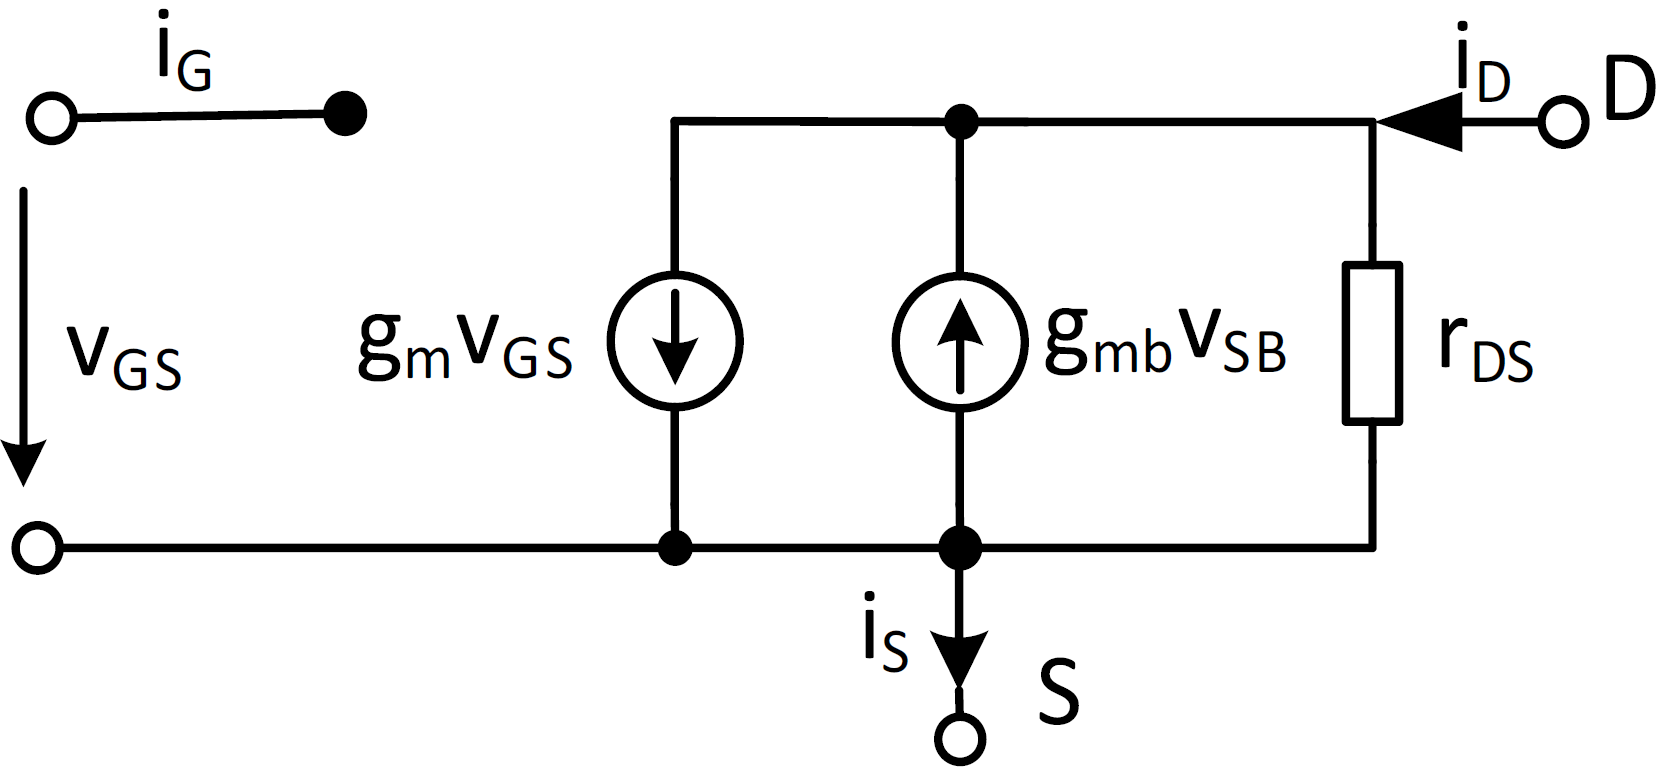
\includegraphics[width=\columnwidth, align=t]{images/02_MOSFET_Pi_Ersatzschaltung.png} Variante aus Skript
    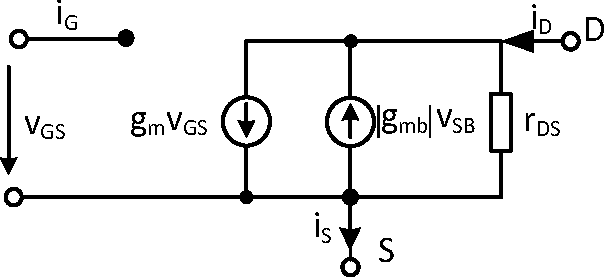
\includegraphics[width=\columnwidth, align=t]{images/02_MOSFET_Pi_Ersatzschaltung_angepasste_Stromrichtung.pdf}
\end{minipage}
\hfill
\begin{minipage}[t]{0.48\columnwidth}
    \raggedright
    \begin{itemize}
        \item Ideale spannungsgesteurte Stromquelle: $I_D = f(V_{\rm GS})$
        \item Berücksichtigung von Kanallängenmodulation: $g_o$ bzw. $r_{\rm DS}$
        \item Berücksichtigung von Body-Effekt: $g_{\rm mb} \cdot V_{\rm SB}$
    \end{itemize}
\end{minipage}


\paragraph{Hochfrequenz}
\label{Hochfrequenz}

\begin{minipage}[t]{0.55\columnwidth}
    % 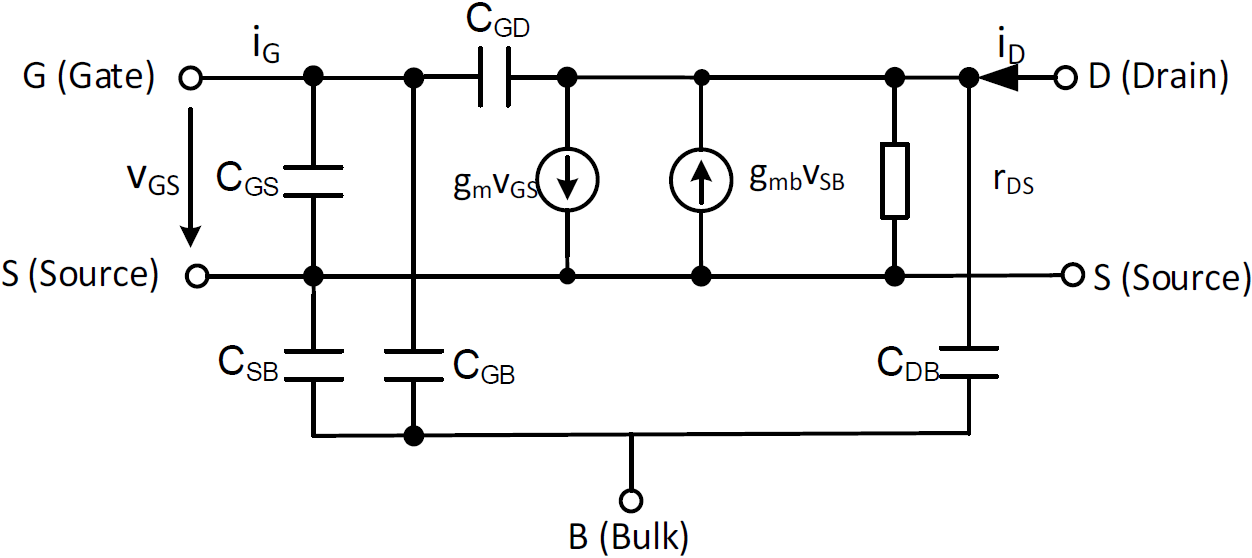
\includegraphics[width=\columnwidth, align=t]{images/02_MOSFET_Kleinsignalersatzschaltung_hochfrequent.png}   Variante aus Skript
    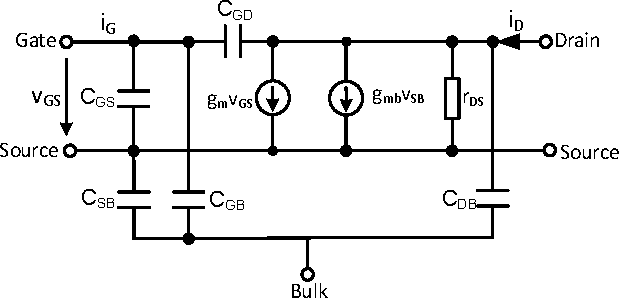
\includegraphics[width=\columnwidth, align=t]{images/02_MOSFET_Kleinsignalersatzschaltung_hochfrequent_angepasste_Stromrichtung.pdf}
\end{minipage}
\hfill
\begin{minipage}[t]{0.44\columnwidth}
    \raggedright
    Wenn Source und Bulk verbunden sind werden
    \begin{itemize}
        \item $C_{\rm GB}$ und $C_{\rm GS}$ parallel geschaltet
        \item $C_{\rm SB}$ kurzgeschlossen.
    \end{itemize}
\end{minipage}


\subsection{Kleinsignalparameter}
\label{Kleinsignalparameter}

Die Kleinsignalparameter bilden eine Vereinfachung (\textbf{Linearisierung}) in einem Arbeitspunkt. 
Sie berechnen sich daher allgemein folgendermassen aus der Ableitung
\[
    g_m                     = \frac{\diff}{\diff V_{\rm GS}} I_D \qquad
    g_o = \frac{1}{r_{\rm DS}}  = \frac{\diff}{\diff V_{\rm DS}} I_D \qquad
    g_{\rm mb}                  = \frac{\diff}{\diff V_{\rm SB}} I_D
\]

Für die beiden Kanalzustände, in welchen Formeln für die Handrechnung verfügbar sind, gibt es auch hier handliche Formeln für die Berechnung der Kleinsignalparameter.

\smallskip

Die Bezeichnung der einzelnen Parameter gilt sowohl für strong inversion als auch für weak inversion.

\medskip

\begin{tabular}{@{}ll@{}}
    $g_m$               & Transkonduktanz (Stromquellenbetrieb) \textrightarrow\ Mass für Verstärkung des Transistors   \\
    $g_{\rm mb}$            & Body-Transkonduktanz \textrightarrow\ Beschreibt Wirkung des Body-Effekts                     \\
    $g_o$               & Ausgangsleitwert (Stromquellenbetrieb) \textrightarrow\ beschreibt Kanallängenmodulation      \\
    $r_{DS \crd{0}}$    & Kleinstmöglicher Ausgangswiderstand bzw. \textbf{Einschaltwiderstand bei} $\bm{V_{\rm DS} = 0}$   \\
                        & \textrightarrow\ Nur im Widerstandsbetrieb interessant
\end{tabular}

\medskip

\textbf{Hinweis:} Folgende Formel gelten für nMOS Transistoren.
Für pMOS Transistoren müssen \textbf{Beträge eingesetzt werden}. Ein Plausibilitäts-Check bzgl. Vorzeichen ist generell ratsam.


\subsubsection{Strong Inversion}

\vspace{-0.3cm}

\[
    \underbrace{ g_m = \mu C_{\rm ox} \frac{W}{L} (V_{\rm GS} - V_T) }_{\text{AP durch } V_{\rm GS} \text{ bestimmt}} \qquad \qquad \qquad
    \underbrace{ g_m = \sqrt{2 \mu C_{\rm ox} \frac{W}{L} I_D} }_{\text{AP durch } I_D \text{ bestimmt}} 
\]

% \[
%     g_{\rm mb} = -g_m \frac{\gamma}{2 \sqrt{\abs{V_{\rm SB}} + \abs{2 \Phi_F}}} = - g_m (n_M - 1)
% \]
% Ungesättigt:
% \[
%     g_o = \frac{1}{r_{\rm DS}} = \mu C_{\rm ox} \frac{W}{L} ((V_{\rm GS} - V_T) - V_{\rm DS})
% \]
% % Gesättigt:
% \[
%     g_o =  \frac{1}{r_{\rm DS}} = \lambda I_{DS, sat} = \frac{I_D}{V_E + V_{\rm DS}} \approx \frac{I_D}{a_E L + V_{\rm DS}}
% \]

\vspace{-0.15cm}

\begin{align*}
                                         g_{\rm mb} &= -g_m \frac{\gamma}{2 \sqrt{\abs{V_{\rm SB}} + \abs{2 \Phi_F}}} = - g_m (n_M - 1)                                     \\
    \text{ \textbf{Ungesättigt:}} \quad     g_o &= \frac{1}{r_{\rm DS}} = \mu C_{\rm ox} \frac{W}{L} ((V_{\rm GS} - V_T) - V_{\rm DS})                                              \\
    \text{ \textbf{Gesättigt:}} \quad       g_o &=  \frac{1}{r_{\rm DS}} = \lambda \cdot I_{\rm DS, sat} = \frac{I_D}{V_E + V_{\rm DS}} \approx \frac{I_D}{a_E \cdot L + V_{\rm DS}}
\end{align*}


\subsubsection{Weak Inversion}

\vspace{-0.3cm}

\[
    g_m = \frac{I_D}{n_M \cdot V_\text{temp}} \quad \text{ \textrightarrow\ Unabhängig von der Geometrie des Transistors!}
\]
% {
%     \raggedleft
%     \textrightarrow\ Unabhängig von der Geometrie des Transistors! \phantom{M}

% }

\vspace{-0.15cm}

\begin{align*}
                                         g_{\rm mb} &= -g_m \frac{\gamma}{2 \sqrt{\abs{V_{\rm SB}} + \abs{2 \Phi_F}}} = - g_m (n_M - 1)                                             \\
    \text{ \textbf{Ungesättigt:}} \quad     g_o &= \frac{1}{r_{\rm DS}} = \frac{V_{\text{temp}}}{I_{D \infty}} \quad \text{ \textrightarrow\ wird meist simuliert}              \\
    \text{ \textbf{Gesättigt:}} \quad       g_o &=  \frac{1}{r_{\rm DS}} = \lambda \cdot  I_{\rm DS, sat} = \frac{I_D}{V_E + V_{\rm DS}}  \approx \frac{I_D}{a_E \cdot L + V_{\rm DS}}
\end{align*}


% \[
%     g_{\rm mb} = -g_m \frac{\gamma}{2 \sqrt{\abs{V_{\rm SB}} + \abs{2 \Phi_F}}} = - g_m (n_M - 1)
% \]
% Ungesättigt:
% \[
%     g_o: \text{Wird üblicherweise simuliert}
% \]
% Gesättigt:
% \[
%     g_o = \frac{1}{r_{\rm DS}} = \lambda I_{DS, sat} = \frac{I_D}{V_E + V_{\rm DS}}
% \]

\subsection{Zusammenhänge}

$g_m$ ist in der Weak Inversion unabhängig der Geometrie. 
Es ist für einen gegebenen Drainstrom möglich, Transistoren, die in Weak Inversion wie auch welche, die in Strong Inversion sind herzustellen.
Das $g_m$ steigt beim Transistor in Strong Inversion 


\subsection{Grosssignalanalyse / AP-Bestimmung}
\label{Grosssignalanalyse / AP-Bestimmung}

Die Grosssignalanalyse untersucht das Verhalten der Schaltung \textbf{im Zeitbereich} und hat folgende Eigenschaften:

\smallskip

\begin{outline}
    \1 Berücksichtigung aller Nichtlinearitäten bei beliebig grossen Signalen
    \1 Simulationen: Transient, DC-Arbeitspunkt, DC-Transferkennlinie
    \1 Handrechnung: Bestimmung des Arbeitspunkts mittels Grosssignalersatzschaltung
\end{outline}


\subsubsection{Grosssignalersatzschaltung}
\label{Grosssignalersatzschaltung}

Zur Bestimmung des \textbf{Arbeitspunkts} bzw. aller Gleichspannungen.
\begin{description}
    \item[AC-Spannungsquellen] durch Kurzschlüsse ersetzen.
    \item[AC-Stromquellen] durch Unterbrüche ersetzen. 
    \item[Kondensatoren] durch Unterbrüche ersetzen.
    \item[Spulen] durch Kurzschlüsse ersetzen.  
\end{description}


\subsection{Kleinsignalanalyse}
\label{Kleinsignalanalyse}

Die Kleinsignalanalyse untersucht das Verhalten der Schaltung \textbf{im Frequenzbereich} und hat folgende Eigenschaften:

\smallskip

\begin{outline}
    \1 Betrachtung von Signalen mit kleiner Amplitude
    \1 Simulationen: AC-Analyse, Transfer-Funktion
    \1 Handrechnung: Rechnung mit linearen Grössen gemäss Kleinsignalersatzschaltung
\end{outline}


\subsubsection{Kleinsignalersatzschaltung}
\label{Kleinsignalersatzschaltung}
Zur Berechnung von Verstärkungsfaktoren und Eingangswiderständen für AC-Signale.

\begin{description}
    \item[DC-Spannungsquellen] durch Kurzschlüsse ersetzen.
    \item[DC-Stromquellen] durch Unterbrüche ersetzen. 
    \item[Nichtlineare Bauteile] durch deren Kleinsignalersatzschaltbild ersetzen.
    \item[Koppel- und Bypass-Kondensatoren] durch Kurzschlüsse ersetzen.  
\end{description}

